\begin{figure}[!h]
  \vskip -0.1cm
  \begin{center}
    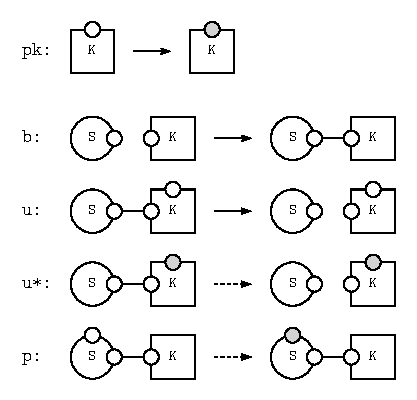
\includegraphics[scale=0.9]{figures/model.pdf}
  \end{center}
  \vskip -0.2cm
  \caption{A motivating toy model. As usual in Kappa, sites not
    mentioned in a rule are left unchanged by it. Instead of naming
    sites, we here identify them by their position on an
    agent. Phosphorylated sites are shown in gray. Firing rates are
    not specified here but dotted arrows indicate \textit{slow}
    reactions, whereas solid arrows indicate \textit{fast} reactions.}
  \label{fig:model}
\end{figure}
